\chapter{Affect Grid Data}\label{app:AG}
Indeholder søjlediagrammer lavet af data indsamlet med \textit{Affect Grid}. På X-aksen står navnene på de individuelle interaktionsopgaver i kronologisk rækkefølge. På X-aksen fornøjelse og ophidselse. Ex1 til Ex7 er betegnelser for programmeringsopgaver udført under Ruby lektionen.


\begin{figure}[h]
\centering
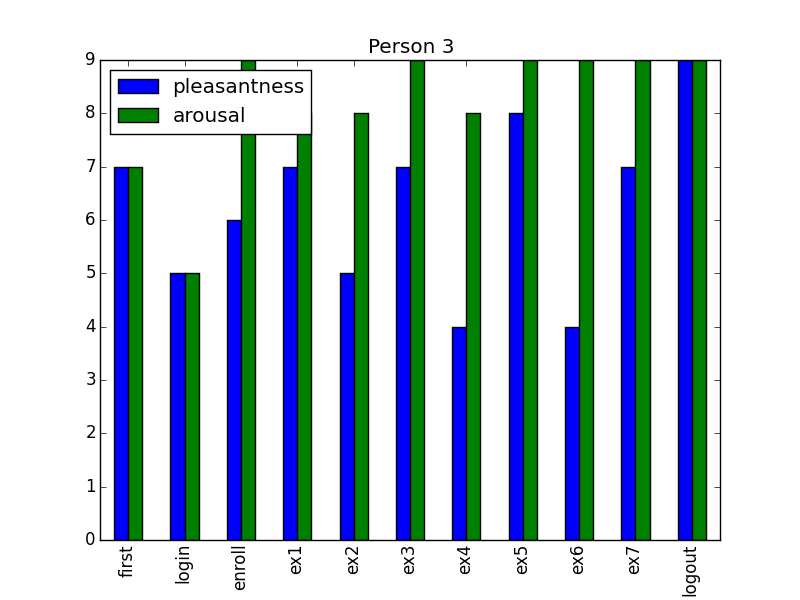
\includegraphics[width=0.8\textwidth]{AGmikael.png}
\caption{Søjlediagram over Affect Grid data fra Testperson 1}
\label{fig:AGMikael}
\end{figure}

\begin{figure}[h]
\centering
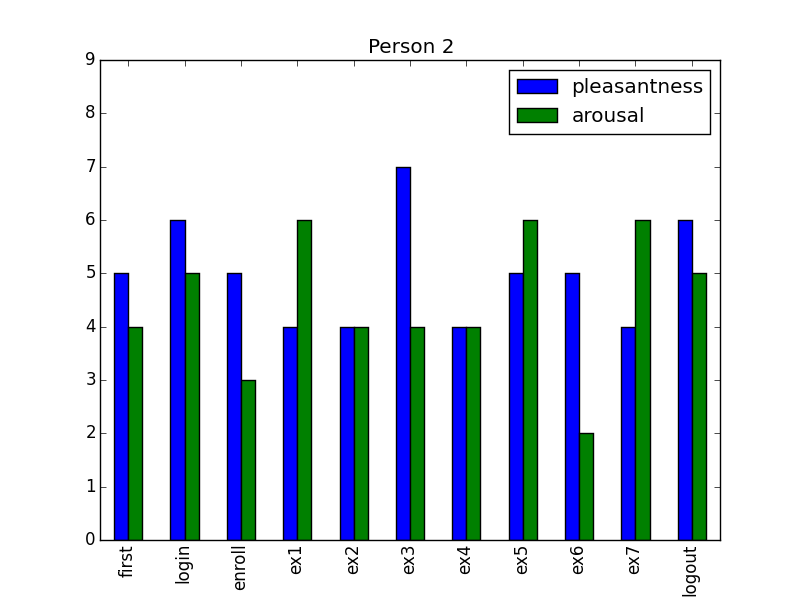
\includegraphics[width=0.8\textwidth]{AGarash.png}
\caption{Søjlediagram over Affect Grid data fra Testperson 2}
\label{fig:AGArash}
\end{figure}

\begin{figure}[h]
\centering
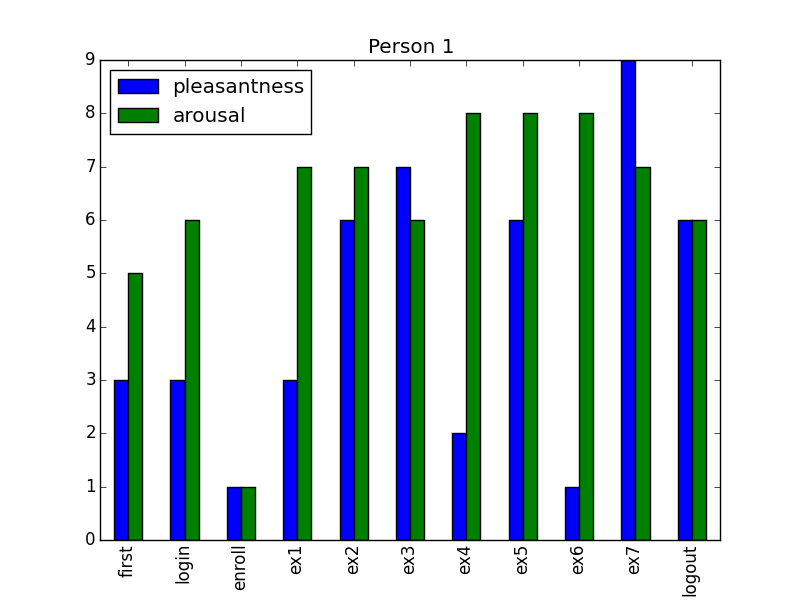
\includegraphics[width=0.8\textwidth]{AGmorten.png}
\caption{Søjlediagram over Affect Grid data fra Testperson 3}
\label{fig:AGMorten}
\end{figure}

\begin{figure}[h]
\centering
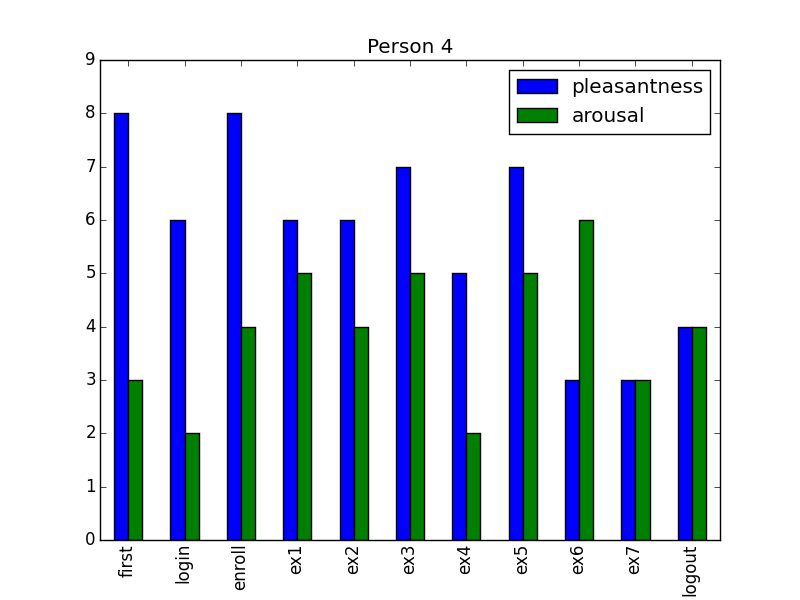
\includegraphics[width=0.8\textwidth]{AGandreas.png}
\caption{Søjlediagram over Affect Grid data fra Testperson 4}
\label{fig:AGAndreas}
\end{figure}